\section{Теоретичні основи е-е}
На відміну від штучно створених мов, наприклад мов програмування чи математичних нотацій,
мови, які ми використовуємо для спілкування, розвивалися з покоління в покоління, постійно
видозмінюючись, а тому досить складно відслідкувати і встановити набір чітких конкретно
визначених правил. Розробка алгоритмів, що дозволяють "розуміти" людські висловлювання
дає змогу покращити велику кількість аспектів взаємодії людини та комп'ютера: передбачення
вводу, розпізнавання тексту, пошук інформації в неструктурованому тексті, переклад з однієї
мови на іншу, аналіз емоційного забарвлення тексту та багато іншого. Створюючи інтерфейси,
що дозволяють людині більш ефективно використовувати комп'ютер, ми прискорюємо
розвиток багатомовного інформаційного суспільства.

\subsection{Методи класифікації даних}

\subsubsection{Проблема класифікації даних}
Задача класифікації – формалізована задача, яка містить множину об’єктів (ситуацій), поділених певним чином на класи. Задана кінцева множина об'єктів для яких відомо, до яких класів вони відносяться. Ця множина називається вибіркою. До якого класу належать інші об'єкти невідомо. Необхідно побудувати такий алгоритм, який буде здатний класифікувати довільний об'єкт з вихідної множини.
Класифікувати об'єкт – означає вказати номер (чи назву) класу, до якого відноситься даний об'єкт.
Класифікація об'єкта – номер або найменування класу, що видається алгоритмом класифікації в результаті його застосування до даного конкретного об'єкту.
В математичній статистиці задачі класифікації називаються також задачами дискретного аналізу. В машинному навчанні завдання класифікації вирішується, як правило, за допомогою методів штучної нейронної мережі при постановці експерименту у вигляді навчання з учителем (supervised machine learning).
Існують також інші способи постановки експерименту – навчання без вчителя (unsupervised learning), але вони використовуються для вирішення іншого завдання – кластеризації або таксономії. У цих завданнях поділ об'єктів навчальної вибірки на класи не задається, і потрібно класифікувати об'єкти тільки на основі їх подібності. У деяких прикладних областях, і навіть у самій математичній статистиці, через близькість завдань часто не відрізняють завдання кластеризації від завдання класифікації.

Деякі алгоритми для вирішення задач класифікації комбінують навчання з учителем і навчання без вчителя, наприклад, одна з версій нейронних мереж Кохонена – мережі векторного квантування, яких навчають способом навчання з учителем.

Прогностичне моделювання – використання статистичних методів для передбачення деякого цільового значення. Зазвичай, мається на увазі передбачення деякої величини в майбутньому, хоча узагальнено це не грає жодної ролі і може бути застосовано до будь-якого типу невідомої події, незалежно від того, коли вона відбулася.
В багатьох випадках задача зводиться до вибору найкращої моделі, що намагається здогадатися результат на основі набору вхідних даних, наприклад визначення того, чи є деякий лист електронної пошти спамом. Моделі можуть використовувати один чи декілька класифікаторів, щоб визначати приналежність даних до деякої множини. Сам термін прогностичної моделі широко перетинається з поняттями машинного навчання в наукових статтях та в контексті розробки програмного забезпечення. В промисловому середовищі даний термін швидше відноситься до поняття прогностичного аналізу.

\subsubsection{Існуючі методи класифікації даних}
В залежності від вхідних даних, для задач класифікації можна виділити такі категорії:

\begin{itemize}  
	\item Характеристичний опис – найпоширеніший випадок. Кожен об'єкт описується набором своїх характеристик, які називаються ознаками. Ознаки можуть бути числовими або нечисловими.
	\item Матриця відстаней між об'єктами. Кожен об'єкт описується відстанями до всіх інших об'єктів навчальної вибірки. З цим типом вхідних даних працюють деякі методи, зокрема, метод найближчих сусідів, метод потенційних функцій.
	\item Часовий ряд або сигнал є послідовність вимірів у часі. Кожен вимір може представлятися числом, вектором, а в загальному випадку – характеристичним описом досліджуваного об'єкта в цей момент часу.
	\item Зображення або відеоряд.
\end{itemize}

Зустрічаються і складніші випадки, коли вхідні дані представляються у вигляді графів, текстів, результатів запитів до бази даних, і т. д. Як правило, вони приводяться до першого або другого випадку шляхом попередньої обробки даних та вилучення характеристик. Щодо класифікації сигналів та зображень, то її також називають розпізнаванням образів.

В залежності від кількості класів, на які розбиваються вхідні дані, отримуємо такий поділ:
\begin{itemize}  
	\item Двокласова класифікація (бінарна класифікація). Найпростіший в технічному відношенні випадок, який служить основою для вирішення складніших завдань.
	\item Багатокласова класифікація. Коли число класів досягає багатьох тисяч (наприклад, при розпізнаванні ієрогліфів або злитого мовлення), завдання класифікації стає істотно важчим.
	\item Непересічні класи.
	\item Пересічні класи. Об'єкт може належати одночасно до декількох класів.
	\item Нечіткі класи. Потрібно визначати ступінь належності об'єкта кожному з класів, звичайно це дійсне число від 0 до 1.
\end{itemize}

Тут реально матеріал з якоїсь книжки і реф на неї \cite{book:1}

\subsubsection{Машинне навчання з учителем}
Машинне навчання - узагальнена назва методів штучної генерації знань з досвіду. Штучна система навчається на прикладах і після закінчення фази навчання може узагальнювати. Тобто система не просто вивчає наведені приклади, а розпізнає певні закономірності в даних для навчання.

Серед багатьох програмних продуктів машинне навчання використовують: системи автоматичного діагностування, розпізнавання шахрайства з кредитними картками, аналіз ринку цінних паперів, класифікація ланцюжків ДНК, розпізнавання мовлення та тексту, автономні системи.

Машинне навчання — розділ штучного інтелекту, має за основу побудову та дослідження систем, які можуть самостійно навчатись з даних. Наприклад, система машинного навчання може бути натренована на електронних повідомленнях для розрізняння спам і не спам-повідомлень. Після навчання вона може бути використана для класифікації нових повідомлень електронної пошти на спам та не-спам папки.

В основі машинного навчання розглядаються уявлення та узагальнення. Представлення даних і функцій оцінки цих даних є частиною всіх систем машинного навчання, наприклад, у наведеному вище прикладі повідомлення по електронній пошті, ми можемо уявити лист як набір англійських слів, просто відмовившись від порядку слів. Існує широкий спектр завдань машинного навчання та успішних застосувань. Оптичне розпізнавання символів, в яких друковані символи розпізнаються автоматично, ґрунтуючись на попередніх прикладах, є класичним прикладом техніки машинного навчання. У 1959 році Артур Самуїл визначив машинне навчання як “Поле дослідження, яке дає комп'ютерам можливість навчатися, не будучи явно запрограмованим” \cite{book:arthur_samuel}.

Практичне використання відбувається, переважно, за допомогою алгоритмів. Різноманітні алгоритми машинного навчання можна грубо поділити за такою схемою:
\begin{itemize}  
	\item Навчання з вчителем – алгоритм вивчає функцію на основі наданих пар вхідних та вихідних даних. При цьому, в процесі навчання, «вчитель» вказує вірні вихідні дані для кожного значення вхідних даних. Одним з розділів навчання з вчителем є машинна класифікація. Такі алгоритми застосовуються для розпізнавання текстів.
	\item Багатокласова класифікація. Коли число класів досягає багатьох тисяч (наприклад, при розпізнаванні ієрогліфів або злитого мовлення), завдання класифікації стає істотно важчим.
	\item Навчання без вчителя.
	\item Пересічні класи. Об'єкт може належати одночасно до декількох класів.
	\item Навчання з закріпленням (англ. reinforcement learning): алгоритм навчається за допомогою тактики нагороди та покарання для максимізації вигоди для агентів (систем до яких належить компонента, що навчається).
\end{itemize}

Узагальнення в цьому контексті є здатність алгоритму для виконання точно на нових, невідомих прикладах після тренування на навчальному наборі даних. Основна мета учня узагальнювати свій досвід.

Також існує поняття інтелектуального аналізу даних, що за своєю природою відрізняється від машинного навчання. Два терміни часто плутають, оскільки вони не рідко використовують ті ж методи і перекриття. Вони можуть бути умовно визначені наступним чином: машинне навчання фокусується на прогноз, заснований на відомих властивостях, витягнутих з навчальних даних. Інтелектуальний аналіз даних (який є кроком виявлення знань у базах даних) фокусується на відкриття (раніше) невідомих властивостей даних.

Ці дві області перекриваються у багатьох відношеннях: інтелектуальний аналіз даних використовує безліч методів машинного навчання, але часто з дещо іншою метою. З іншого боку, машинне навчання також використовує методи інтелектуального аналізу такі як "неконтрольоване навчання" або як попередній крок оброблення для покращення точності навчальної системи. Велика частина плутанини відбувається з основних припущень: в машинному навчанні, виконання, як правило, оцінюється по відношенню до здатності відтворювати відомі знання, в той час як в інтелектуальному аналізі даних ключовим завданням є виявлення раніше невідомого знання. Необізнаний (неконтрольований) метод, який обчислюється по відношенню до відомих знань, буде легко перевершений керованими методами. В той час в типових ІАД завданнях, керовані методи не можуть бути використані через відсутність попередньої підготовки даних.

Деякі системи машинного навчання намагаються усунути необхідність в людській інтуїції під час аналізування даних, а інші обирають спільний підхід між людиною і машиною. Людська інтуїція не може бути повністю виключена, так як конструктору системи необхідно вказати, як дані повинні бути представлені і які механізми будуть використовуватися для пошуку характеристик даних.

Навчання з підкріпленням — це галузь машинного навчання натхненна біхевіористською психологією, що займається питанням про те, які дії мають виконувати програмні агенти в певному середовищі задля максимізації деякого уявлення про сукупну винагороду. Через свою загальність, дана проблема вивчається, вивчається багатьма іншими дисциплінами, такими як теорія ігор, теорія управління, дослідження операцій, теорія інформації, оптимізація на основі моделювання, багатоагентні системи, колективний інтелект, статистика та генетичні алгоритми. Галузь, що займається навчанням з підкріпленням, також називається наближеним динамічним програмуванням. Попри те, що проблема навчання з підкріпленням, вивчалась теорією оптимального управління, більшість досліджень стосувались саме існування оптимальних рішень та їх характеристики, а не навчання чи наближених аспектів. В економіці та теорії ігор, навчання з підкріпленням може використовуватись для пояснення того, як при обмеженій раціональності може виникати рівновага.

Навчання з учителем (англ. supervised learning) є одним із способів машинного навчання, в ході якого випробувана система примусово навчається за допомогою наявної множини прикладів «стимул-реакція» з метою визначення «реакції» для «стимулів», які не належать наявній множині прикладів. 

Між входами та еталонними виходами (стимул-реакція) може існувати деяка залежність, але вона невідома. Відома лише кінцева сукупність прецедентів – пар «стимул-реакція», звана навчальною вибіркою. На основі цих даних потрібно відновити залежність (побудувати модель відносин стимул-реакція, придатних для прогнозування), тобто побудувати алгоритм, здатний для будь-якого об'єкта видати досить точну відповідь. Для вимірювання точності відповідей, так само як і в навчанні на прикладах, може вводитися функціонал якості.

Задача машинного навчання може бути представлена у вигляді експерименту. Даний експеримент являє собою окремий випадок кібернетичного експерименту зі зворотним зв'язком. Постановка даного експерименту припускає наявність експериментальної системи, методу навчання і методу випробування системи або вимірювання характеристик.

Експериментальна система у свою чергу складається з випробовуваної (використовуваної) системи, простору стимулів одержуваних із зовнішнього середовища та системи управління підкріпленням (регулятора внутрішніх параметрів). В якості системи управління підкріпленням може бути використано автоматичний пристрій, що регулюють (наприклад, термостат), або людину-оператора (вчитель), здатну реагувати на реакції випробовуваної системи і стимули зовнішнього середовища шляхом застосування особливих правил підкріплення, що змінюють стан пам'яті системи.

Розрізняють два варіанти: (1) коли реакція випробовуваної системи не змінює стан зовнішнього середовища, і (2) коли реакція системи змінює стимули зовнішнього середовища. На рис. \ref{fig:experiment_system} зображено загальний вигляд такої експериментальної системи.
\begin{figure}[h!]
  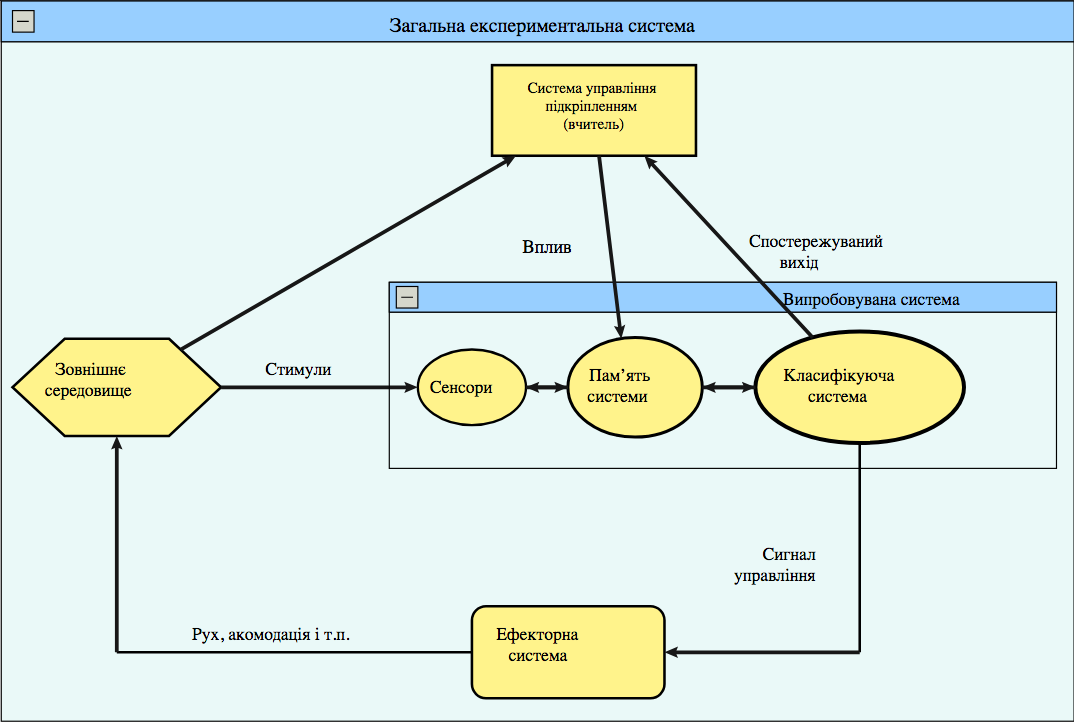
\includegraphics[width=\linewidth]{figures/fig_system.png}
  \caption{Експериментальна система для навчання з учителем}
  \label{fig:experiment_system}
\end{figure}

В залежності від результуючих даних, отриманих від системи, можна виділити такі категорії класифікуючих систем:
\begin{itemize}  
	\item Множина можливих відповідей нескінчення (відповіді є дійсними числами або векторами). В даному випадку говорять про задачі регресії та апроксимації.
	\item Множина відповідей звичайна – задача класифікації та розпізнавання образів.
	\item Відповіді характеризують майбутню поведінку процесу або явища. В цьому випадку мова йде про задачі прогнозування (прогностичне моделювання).
\end{itemize}


In text classification, we are given a description
$\mathbb{X}$ of a document, where $\mathbb{X}$ is the document space ; and a fixed set
of classes  $\mathbb{C}$ Classes are also called categories or
labels . Typically, the document space  $\mathbb{X}$ is some type of high-dimensional space,
and the classes are human defined for the needs of an application, as in the examples China
and documents that talk about multicore computer chips above.

\subsection{Exploratory data analysis}
Візуалізація для наступних цілей:
* Комунікативна
- представлення даних та ідей
- проінформувати
- підтримати і аргументувати
- вплинути і переконати
* Дослідницька
- вивчити (дослідити) дані
- проаналізувати ситуацію
- визначити наступні кроки
- прийняти рішення стосовно деякого питання

\begin{equation}
    \label{simple_equation}
    \alpha = \sqrt{ \beta }
\end{equation}

\subsection{Класифікація тексту}
Метою класифікації текстів є розподіл документів на групи наперед визначених категорій. *-*


\subsection{Учи матчасть}
Результати показують, що стабільно показують чудові результати для завдань класифікації
текстів, суттєво перевищуючи показники інших методів.

